\documentclass[11pt,letterpaper]{article}
\usepackage[lmargin=1in,rmargin=1in,tmargin=1in,bmargin=1in]{geometry}
\usepackage{../style/homework}
\usepackage{../style/commands}
\setbool{quotetype}{true} % True: Side; False: Under
\setbool{hideans}{true} % Student: True; Instructor: False

% -------------------
% Content
% -------------------
\begin{document}

\homework{5: Due 01/11}{I just want to lie on the beach and eat hot dogs. That's all I've ever wanted.}{Kevin Malone, The Office}

% Problem 1
\problem{10} Determine if the following function is linear. Explain why or why not.
	\begin{table}[!ht]
	\centering
	\begin{tabular}{c|c}
	$x$ & $f(x)$ \\ \hline
	$1.2$ & $7.16$ \\
	$2.8$ & $12.39$ \\
	$4.4$ & $16.12$ \\
	$6.0$ & $22.13$ \\
	$7.6$ & $25.08$
	\end{tabular}
	\end{table}



\newpage



% Problem 2
\problem{10} A linear function has a table whose values are given below. Find the equation of the linear function. Be sure to specify the slope and $y$-intercept.
	\begin{table}[!ht]
	\centering
	\begin{tabular}{c|c}
	$x$ & $f(x)$ \\ \hline
	$2$ & $20$ \\
	$7$ & $-5$ \\
	$12$ & $-30$ \\
	$17$ & $-55$
	\end{tabular}
	\end{table}



\newpage



% Problem 3
\problem{10} Plot the linear function $y= \frac{3}{2} x - 4$ using the ``two-point'' method. \pspace
	\[
	\fbox{
	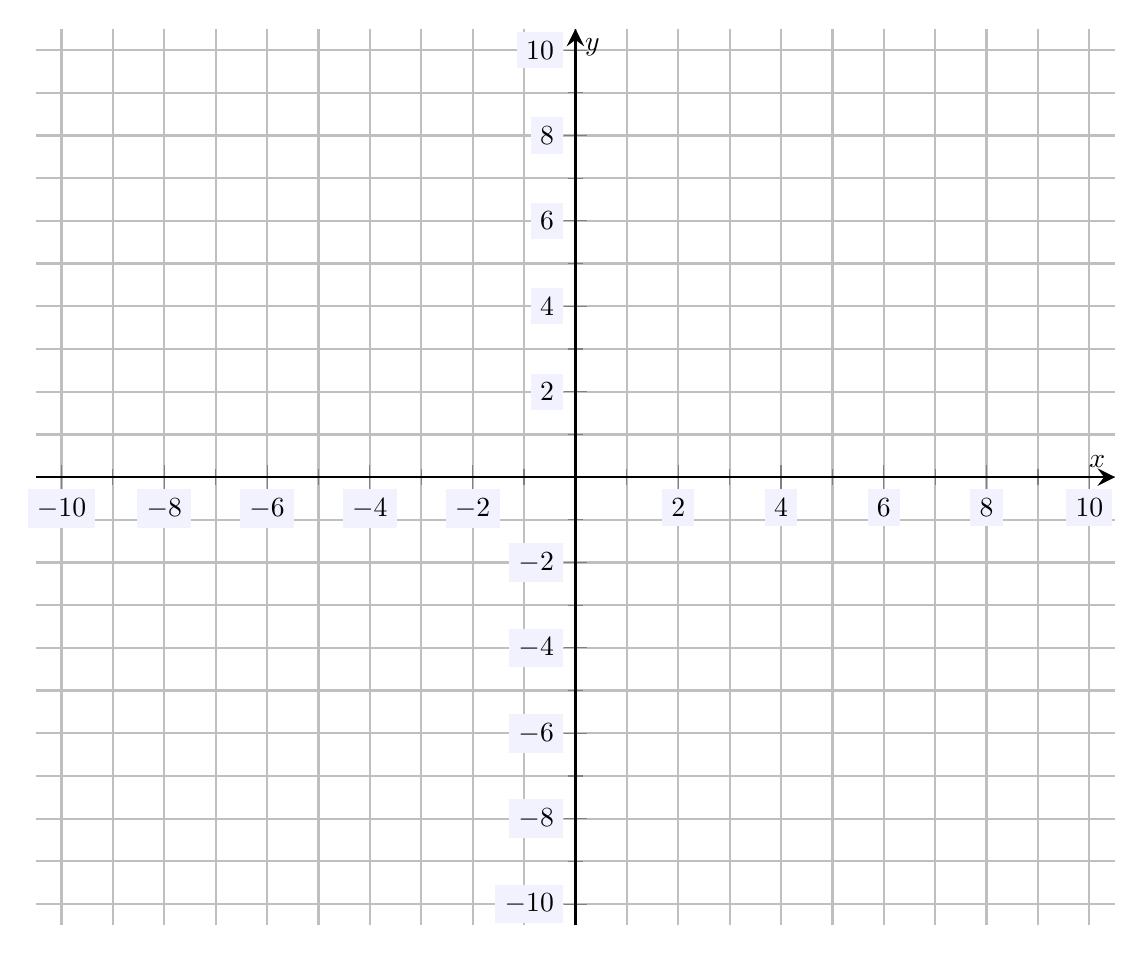
\begin{tikzpicture}[scale=2,every node/.style={scale=0.5}]
	\begin{axis}[
	grid=both,
	axis lines=middle,
	ticklabel style={fill=blue!5!white},
	xmin= -10.5, xmax=10.5,
	ymin= -10.5, ymax=10.5,
	xtick={-10,-8,-6,-4,-2,0,2,4,6,8,10},
	ytick={-10,-8,-6,-4,-2,0,2,4,6,8,10},
	minor tick = {-10,-9,...,10},
	xlabel=\(x\),ylabel=\(y\),
	]
	\end{axis}
	\end{tikzpicture}
	}
	\]



\newpage



% Problem 4 
\problem{10} Plot the linear function $y= -\frac{1}{2} x + 3$ using the ``slope'' method. 
	\[
	\fbox{
	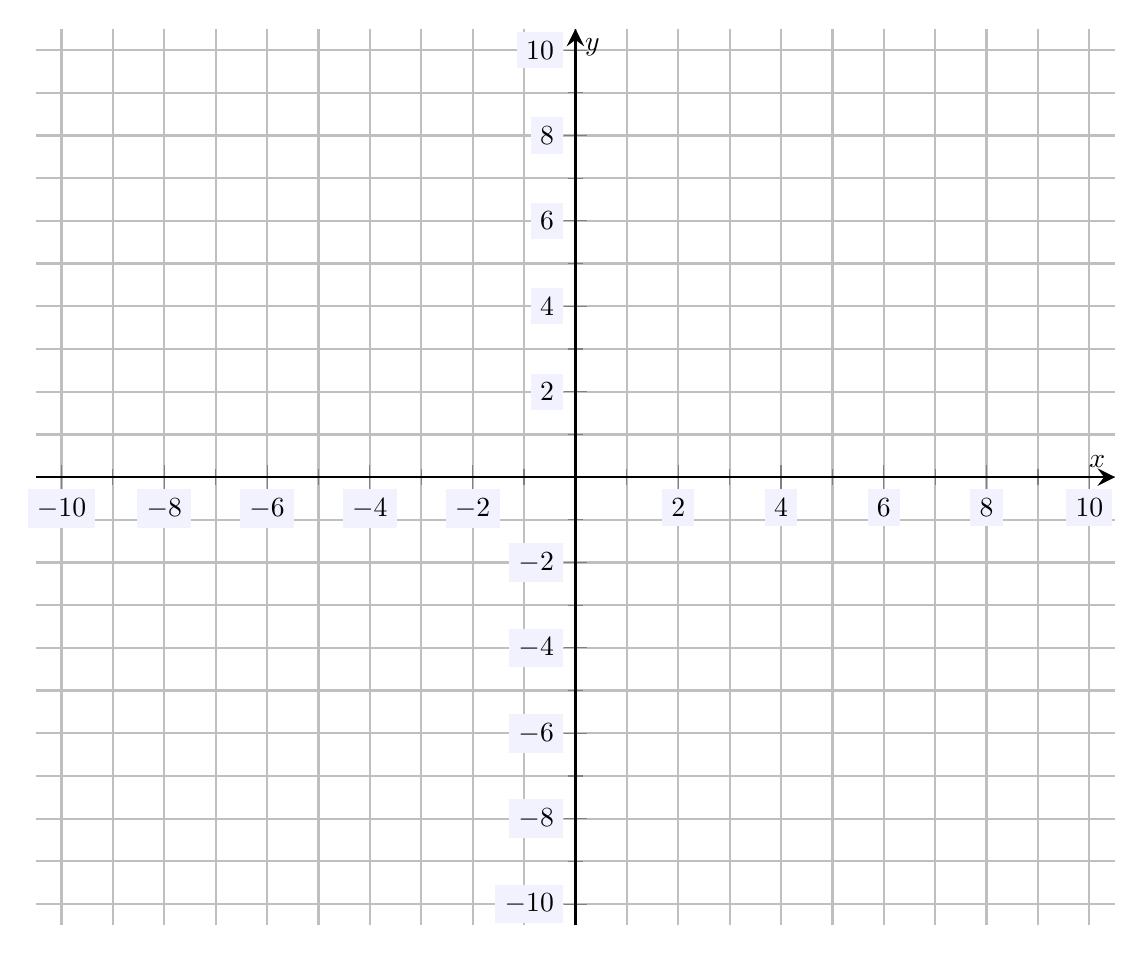
\begin{tikzpicture}[scale=2,every node/.style={scale=0.5}]
	\begin{axis}[
	grid=both,
	axis lines=middle,
	ticklabel style={fill=blue!5!white},
	xmin= -10.5, xmax=10.5,
	ymin= -10.5, ymax=10.5,
	xtick={-10,-8,-6,-4,-2,0,2,4,6,8,10},
	ytick={-10,-8,-6,-4,-2,0,2,4,6,8,10},
	minor tick = {-10,-9,...,10},
	xlabel=\(x\),ylabel=\(y\),
	]
	\end{axis}
	\end{tikzpicture}
	}
	\]



\newpage



% Problem 5
\problem{10} Suppose water is draining from a tank. The number of gallons of water in the tank $t$ hours from now is given by $W(t)= 567.8 - 24.1t$.
\begin{enumerate}[(a)]
\item Is $W(t)$ linear? Explain.
\item What is the slope of $W(t)$? Interpret the slope.
\item Explain how we can know that water is draining from the tank using (b).
\item What is the $y$-intercept for $W(t)$? Interpret this intercept. 
\item Sketch a plot of $W(t)$ and estimate when the tank will be completely empty. 
\end{enumerate}



\newpage



% Problem 6
\problem{10} Consider the linear equation $12x - 2y= 56$. 
\begin{enumerate}[(a)]
\item Solve the linear equation for $y$. 
\item Determine the slope and $y$-intercept for the corresponding line.
\item Interpret the slope in at least two different ways. 
\end{enumerate}



\newpage



% Problem 7
\problem{10} Consider the linear equation $7.6x + 14.9y= 429.1$. 
\begin{enumerate}[(a)]
\item Solve the linear equation for $y$. 
\item Determine the slope and $y$-intercept for the corresponding line.
\item Interpret the slope in at least two different ways. 
\end{enumerate}



\newpage



% Problem 8
\problem{10} Consider the line given by $y= -\frac{7}{6}x + 5$.
\begin{enumerate}[(a)]
\item Put the line in standard form.
\item Is the point $(-6, 10)$ on the line? Explain.
\item Is the point $(12, -9)$ on the line? Explain. 
\end{enumerate}



\newpage



% Problem 9
\problem{10} Find the equation of the line with slope $-\frac{15}{4}$ and $y$-intercept $(0, -8)$. \pspace



\newpage



% Problem 10
\problem{10} Find the equation of the line with slope $5$ passing through the point $(-3, 10)$. \pspace


\end{document}